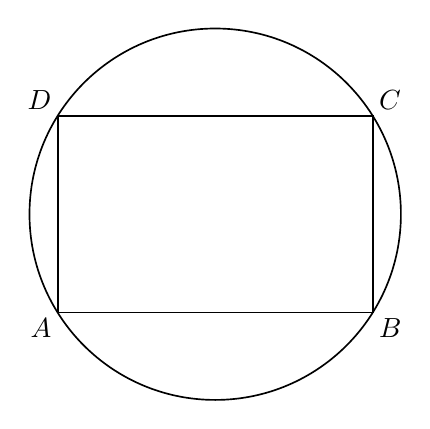
\begin{tikzpicture}[x=1cm,y=1cm,line width=.6pt,font=\normalsize]
\coordinate (O) at (0,0);
\coordinate (A) at (-2,-1.25);
\coordinate (B) at (2,-1.25);
\coordinate (C) at (2,1.25);
\coordinate (D) at (-2,1.25);
\draw (O) circle[radius=2.3585cm];
\draw (A)--(B)--(C)--(D)--cycle;
\node[below left=2pt,inner sep=0pt] at (A) {$A$};
\node[below right=2pt,inner sep=0pt] at (B) {$B$};
\node[above right=2pt,inner sep=0pt] at (C) {$C$};
\node[above left=2pt,inner sep=0pt] at (D) {$D$};
\end{tikzpicture}
